\documentclass{article}
\usepackage{adjustbox}
\usepackage{graphicx}
\usepackage{geometry}
\usepackage{dcolumn}
 \geometry{
 a4paper,
 total={170mm,257mm},
 left=10mm,
 top=10mm
 }

\title{Reliability Analysis for Serbian Respondents}
\date{July 2023}

\begin{document}

\subsubsection*{Reliability Analysis Overview}

For constructs, we refer to $construct\_variable$ field. All constructs are composed of either Likert scale variables or Binary scale variables and not both. For the first step of the reliability analysis, we test for the internal consistency of each construct using Cronbach's alpha. Table \ref{tbl:constructs_alpha_matrix} summarizes raw and standardized alpha of each construct along with the number of variables in it.

\subsubsection*{Cronbach's Alpha}

\begin{itemize}
    \item \textbf{High reliability} : constructs that have a reliability of over (or close to) 0.7, indicating good internal consistency
    \begin{enumerate}
        \item $dev\_knw\_recog$
        \item $parent\_knw$
        \item $practices\_agree$
        \item $practices\_hostility$
    \end{enumerate}
    \item \textbf{Low reliability} : constructs with reliability much lower than 0.7 indicating poor internal consistency
    \begin{enumerate}
        \item $dev\_knw\_concern\_0\_2$
        \item $dev\_knw\_concern\_3\_6$
        \item $health\_knw$
        \item $practices\_24$
        \item $caregiver\_well\_being$
    \end{enumerate}

% Table created by stargazer v.5.2.3 by Marek Hlavac, Social Policy Institute. E-mail: marek.hlavac at gmail.com
% Date and time: Tue, Sep 19, 2023 - 22:12:00
% Requires LaTeX packages: dcolumn 
\begin{table}[!htbp] \centering 
  \caption{} 
  \label{tbl:constructs_alpha_matrix_bulgaria} 
\begin{tabular}{@{\extracolsep{5pt}} D{.}{.}{-2} D{.}{.}{-2} D{.}{.}{-2} D{.}{.}{-2} } 
\\[-1.8ex]\hline 
\hline \\[-1.8ex] 
\multicolumn{1}{c}{construct} & \multicolumn{1}{c}{variable count} & \multicolumn{1}{c}{raw.alpha} & \multicolumn{1}{c}{std.alpha} \\ 
\hline \\[-1.8ex] 
\multicolumn{1}{c}{health\_knw} & \multicolumn{1}{c}{2} & \multicolumn{1}{c}{0.5} & \multicolumn{1}{c}{0.53} \\ 
\multicolumn{1}{c}{dev\_knw\_recog} & \multicolumn{1}{c}{4} & \multicolumn{1}{c}{0.78} & \multicolumn{1}{c}{0.78} \\ 
\multicolumn{1}{c}{confidence} & \multicolumn{1}{c}{2} & \multicolumn{1}{c}{0.81} & \multicolumn{1}{c}{0.81} \\ 
\multicolumn{1}{c}{attitude} & \multicolumn{1}{c}{1} & \multicolumn{1}{c}{} & \multicolumn{1}{c}{} \\ 
\multicolumn{1}{c}{caregiver\_well\_being} & \multicolumn{1}{c}{3} & \multicolumn{1}{c}{0.42} & \multicolumn{1}{c}{0.42} \\ 
\multicolumn{1}{c}{was\_breastfed} & \multicolumn{1}{c}{1} & \multicolumn{1}{c}{} & \multicolumn{1}{c}{} \\ 
\multicolumn{1}{c}{practices\_24} & \multicolumn{1}{c}{6} & \multicolumn{1}{c}{0.5} & \multicolumn{1}{c}{0.58} \\ 
\multicolumn{1}{c}{practices\_agree} & \multicolumn{1}{c}{4} & \multicolumn{1}{c}{0.53} & \multicolumn{1}{c}{0.55} \\ 
\multicolumn{1}{c}{practices\_hostility} & \multicolumn{1}{c}{4} & \multicolumn{1}{c}{0.78} & \multicolumn{1}{c}{0.78} \\ 
\hline \\[-1.8ex] 
\end{tabular} 
\end{table} 
 

    \item For these constructs with low reliability, we look at the reliability with variables dropped.
\end{itemize}


\subsubsection*{Reliability after variable is dropped}

For each construct in Table \ref{tbl:alpha_drop}, we see how the reliability changes if a variable from that construct is dropped.
\begin{itemize}
    \item $caregiver\_well\_being$ : Any variable dropped leads to lower reliability than with all variables included.
    \item $dev\_knw\_concern\_0\_2$ : Dropping variables $scribble$ and $say\_name\_age$ leads to a higher reliability. 
    \begin{itemize}
        \item However, even after dropping either of these variables, the reliability would be 0.03-0.05.
        \item It appears that the variables under construct Development Knowledge Concern (0-2) are generally uncorrelated or negatively correlated.
        \item This might be because respondents have partial knowledge of children's development and might get only one or a few of the questions correct.
    \end{itemize} 
    
 
    \item $dev\_knw\_concern\_3\_6$ : The construct's internal consistency can be improved by dropping variable $alphabet$.

    \item $health\_knw$ : Any variable dropped leads to lower reliability than with all variables included.
\end{itemize}


% Table created by stargazer v.5.2.3 by Marek Hlavac, Social Policy Institute. E-mail: marek.hlavac at gmail.com
% Date and time: Tue, Sep 19, 2023 - 22:12:00
% Requires LaTeX packages: dcolumn 
\begin{table}[!htbp] \centering 
  \caption{Reliability if variable is dropped - Bulgaria} 
  \label{tbl:alpha_drop_bulgaria} 
\begin{tabular}{@{\extracolsep{5pt}} D{.}{.}{-2} D{.}{.}{-2} D{.}{.}{-2} D{.}{.}{-2} D{.}{.}{-2} } 
\\[-1.8ex]\hline 
\hline \\[-1.8ex] 
\multicolumn{1}{c}{construct} & \multicolumn{1}{c}{variable.dropped} & \multicolumn{1}{c}{increment} & \multicolumn{1}{c}{raw\_alpha} & \multicolumn{1}{c}{std.alpha} \\ 
\hline \\[-1.8ex] 
\multicolumn{1}{c}{caregiver\_well\_being} & \multicolumn{1}{c}{parenting\_stress\_1} & \multicolumn{1}{c}{-0.14} & \multicolumn{1}{c}{0.28} & \multicolumn{1}{c}{0.29} \\ 
\multicolumn{1}{c}{caregiver\_well\_being} & \multicolumn{1}{c}{parenting\_stress\_2} & \multicolumn{1}{c}{-0.03} & \multicolumn{1}{c}{0.39} & \multicolumn{1}{c}{0.39} \\ 
\multicolumn{1}{c}{caregiver\_well\_being} & \multicolumn{1}{c}{personal\_needs} & \multicolumn{1}{c}{-0.13} & \multicolumn{1}{c}{0.29} & \multicolumn{1}{c}{0.30} \\ 
\multicolumn{1}{c}{confidence} & \multicolumn{1}{c}{confidence\_deal\_emotions} & \multicolumn{1}{c}{-0.18} & \multicolumn{1}{c}{0.63} & \multicolumn{1}{c}{0.68} \\ 
\multicolumn{1}{c}{confidence} & \multicolumn{1}{c}{confidence\_respond\_misbehave} & \multicolumn{1}{c}{-0.08} & \multicolumn{1}{c}{0.73} & \multicolumn{1}{c}{0.68} \\ 
\multicolumn{1}{c}{dev\_knw\_recog} & \multicolumn{1}{c}{know\_social\_emotional\_dev} & \multicolumn{1}{c}{-0.03} & \multicolumn{1}{c}{0.75} & \multicolumn{1}{c}{0.76} \\ 
\multicolumn{1}{c}{dev\_knw\_recog} & \multicolumn{1}{c}{know\_cog\_dev} & \multicolumn{1}{c}{-0.05} & \multicolumn{1}{c}{0.73} & \multicolumn{1}{c}{0.74} \\ 
\multicolumn{1}{c}{dev\_knw\_recog} & \multicolumn{1}{c}{know\_phys\_dev} & \multicolumn{1}{c}{-0.10} & \multicolumn{1}{c}{0.68} & \multicolumn{1}{c}{0.68} \\ 
\multicolumn{1}{c}{dev\_knw\_recog} & \multicolumn{1}{c}{know\_lang\_dev} & \multicolumn{1}{c}{-0.05} & \multicolumn{1}{c}{0.73} & \multicolumn{1}{c}{0.73} \\ 
\multicolumn{1}{c}{health\_knw} & \multicolumn{1}{c}{know\_which\_vaccine} & \multicolumn{1}{c}{ 0.02} & \multicolumn{1}{c}{0.52} & \multicolumn{1}{c}{0.36} \\ 
\multicolumn{1}{c}{health\_knw} & \multicolumn{1}{c}{know\_when\_vaccine} & \multicolumn{1}{c}{-0.25} & \multicolumn{1}{c}{0.25} & \multicolumn{1}{c}{0.36} \\ 
\multicolumn{1}{c}{practices\_24} & \multicolumn{1}{c}{past\_24h\_read} & \multicolumn{1}{c}{-0.07} & \multicolumn{1}{c}{0.43} & \multicolumn{1}{c}{0.54} \\ 
\multicolumn{1}{c}{practices\_24} & \multicolumn{1}{c}{past\_24h\_stories} & \multicolumn{1}{c}{-0.01} & \multicolumn{1}{c}{0.49} & \multicolumn{1}{c}{0.58} \\ 
\multicolumn{1}{c}{practices\_24} & \multicolumn{1}{c}{past\_24h\_sing} & \multicolumn{1}{c}{-0.03} & \multicolumn{1}{c}{0.47} & \multicolumn{1}{c}{0.55} \\ 
\multicolumn{1}{c}{practices\_24} & \multicolumn{1}{c}{past\_24h\_outside} & \multicolumn{1}{c}{-0.06} & \multicolumn{1}{c}{0.44} & \multicolumn{1}{c}{0.50} \\ 
\multicolumn{1}{c}{practices\_24} & \multicolumn{1}{c}{past\_24h\_play} & \multicolumn{1}{c}{-0.07} & \multicolumn{1}{c}{0.43} & \multicolumn{1}{c}{0.47} \\ 
\multicolumn{1}{c}{practices\_24} & \multicolumn{1}{c}{past\_24h\_draw} & \multicolumn{1}{c}{-0.02} & \multicolumn{1}{c}{0.48} & \multicolumn{1}{c}{0.56} \\ 
\multicolumn{1}{c}{practices\_agree} & \multicolumn{1}{c}{laugh\_together} & \multicolumn{1}{c}{-0.11} & \multicolumn{1}{c}{0.42} & \multicolumn{1}{c}{0.44} \\ 
\multicolumn{1}{c}{practices\_agree} & \multicolumn{1}{c}{joke\_with\_child} & \multicolumn{1}{c}{-0.04} & \multicolumn{1}{c}{0.49} & \multicolumn{1}{c}{0.51} \\ 
\multicolumn{1}{c}{practices\_agree} & \multicolumn{1}{c}{smile\_around\_child} & \multicolumn{1}{c}{-0.09} & \multicolumn{1}{c}{0.44} & \multicolumn{1}{c}{0.45} \\ 
\multicolumn{1}{c}{practices\_agree} & \multicolumn{1}{c}{play\_on\_floor} & \multicolumn{1}{c}{-0.04} & \multicolumn{1}{c}{0.49} & \multicolumn{1}{c}{0.51} \\ 
\multicolumn{1}{c}{practices\_hostility} & \multicolumn{1}{c}{snap\_at\_child} & \multicolumn{1}{c}{-0.08} & \multicolumn{1}{c}{0.70} & \multicolumn{1}{c}{0.70} \\ 
\multicolumn{1}{c}{practices\_hostility} & \multicolumn{1}{c}{lose\_patience\_punish} & \multicolumn{1}{c}{-0.08} & \multicolumn{1}{c}{0.70} & \multicolumn{1}{c}{0.69} \\ 
\multicolumn{1}{c}{practices\_hostility} & \multicolumn{1}{c}{threaten} & \multicolumn{1}{c}{-0.10} & \multicolumn{1}{c}{0.68} & \multicolumn{1}{c}{0.68} \\ 
\multicolumn{1}{c}{practices\_hostility} & \multicolumn{1}{c}{make\_fun\_of} & \multicolumn{1}{c}{ 0.03} & \multicolumn{1}{c}{0.81} & \multicolumn{1}{c}{0.81} \\ 
\hline \\[-1.8ex] 
\end{tabular} 
\end{table} 
 
 

% \subsubsection*{Factor Analysis}

% For the factor analysis, I drop all questions that are shown to only some of the respondents based on selection criteria and have missing values for other respondents that were not shown the question. On the remaining variables, I run a principal component analysis. I infer the number of factors from a scree plot. Image \ref{img: variables loadings on factors} and Table \ref{tbl:all_variables_loadings} display the loadings of the different variables on the first 7 factors. 

% Generally, most variables that belong to the same construct load on the same principal components. Some observations - 
% \begin{itemize}
%     \item $know\_social\_emotional\_dev$, $know\_cog\_dev$, $know\_phy\_dec$, $know\_lang\_dev$ all load on factor 2
%     \item $confidence\_deal\_emotions$ and $confidence\_respond\_misbehave$ load on factor 5
%     \item $decrease\_stress$ and $improve\_family$ load on factor 6
%     \item $past\_24h\_read$, $past\_24h\_stories$, $past\_24h\_draw$, all load on factor 3. However, $past\_24h\_outside$ and $past\_24h\_play$ load on factor 7 more strongly. In fact, $past\_24h\_outside$ and $past\_24h\_draw$ are measuring different ends of the same factor.
%     \item $snap\_at\_child$, $lose\_patience\_punish$, $threaten$, $make\_fun\_of$ all load on factor 5 and measure the opposite end of the factor that drives confidence in dealing with emotions.
%     \item $laugh\_together$, $joke\_with\_child$, $play\_on\_floor$, $smile\_around\_child$ and $play\_on\_floor$ all load on factor 1.
% \end{itemize}

% \textbf{Based on the above, I would infer that }
% \begin{itemize}
%     \item factor 1 represents knowledgeable parenting practices with child
%     \item factor 2 represents cognitive development knowledge
%     \item factor 3 represents the regularity of positive parenting practices
%     \item factor 4 represents positive parenting practices
%     \item factor 5 confidence in dealing with emotion and the absence of which results in stressful and negative behavior
%     \item factor 6 self-care or proactive behavior - these two variables are currently separate constructs but can be grouped as one.
%     \item factor 7 represents past 24 hours outside vs past 24 hours draw. This could represent discipline vs a carefree attitude. More generally, it is plausible that parents that played outside with their children in the last 24 hours did not also draw with their children in the same time frame. A parent that did one would not do the other but we are not interested in that difference. Would it suffice to have a measure where parents did any one of the two? 

% \end{itemize}

% \begin{figure}[h!]

% \caption{Principal Component Analysis - Variables Loadings on Factors}
% \label{img: variables loadings on factors}
% \vspace{1em}
% \centering
% 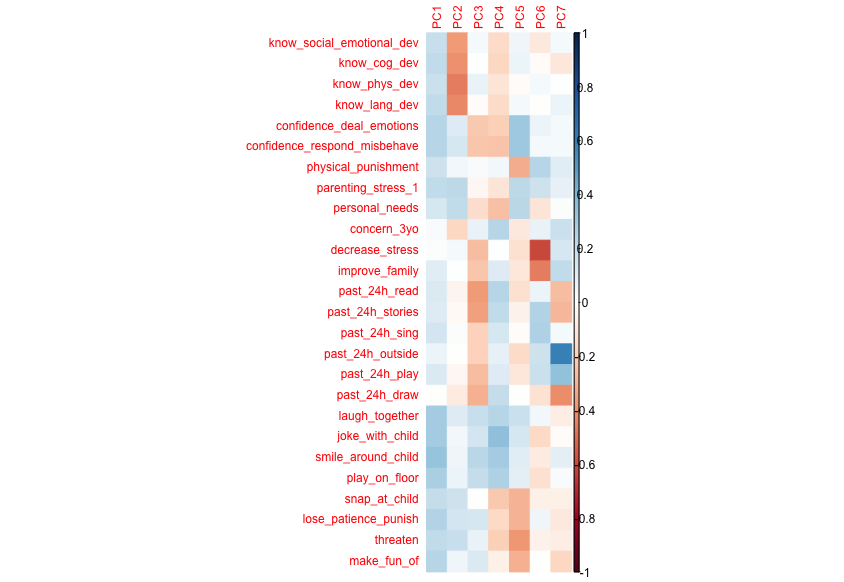
\includegraphics[scale=0.8]{all_variable_loadings_img.png}
% \end{figure}

% 
% Table created by stargazer v.5.2.3 by Marek Hlavac, Social Policy Institute. E-mail: marek.hlavac at gmail.com
% Date and time: Mon, Aug 07, 2023 - 22:05:28
% Requires LaTeX packages: dcolumn 
\begin{table}[!htbp] \centering 
  \caption{} 
  \label{tbl:all_variables_loadings} 
\begin{tabular}{@{\extracolsep{5pt}} D{.}{.}{-2} D{.}{.}{-2} D{.}{.}{-2} D{.}{.}{-2} D{.}{.}{-2} D{.}{.}{-2} D{.}{.}{-2} D{.}{.}{-2} } 
\\[-1.8ex]\hline 
\hline \\[-1.8ex] 
\multicolumn{1}{c}{} & \multicolumn{1}{c}{PC1} & \multicolumn{1}{c}{PC2} & \multicolumn{1}{c}{PC3} & \multicolumn{1}{c}{PC4} & \multicolumn{1}{c}{PC5} & \multicolumn{1}{c}{PC6} & \multicolumn{1}{c}{PC7} \\ 
\hline \\[-1.8ex] 
\multicolumn{1}{c}{know\_social\_emotional\_dev} & 0.19 & -0.38 & 0.03 & -0.16 & 0.05 & -0.10 & 0.03 \\ 
\multicolumn{1}{c}{know\_cog\_dev} & 0.21 & -0.41 & 0 & -0.18 & 0.06 & -0.02 & -0.11 \\ 
\multicolumn{1}{c}{know\_phys\_dev} & 0.18 & -0.46 & 0.07 & -0.12 & -0.02 & 0.03 & 0 \\ 
\multicolumn{1}{c}{know\_lang\_dev} & 0.21 & -0.43 & -0.02 & -0.16 & 0.03 & -0.01 & 0.06 \\ 
\multicolumn{1}{c}{confidence\_deal\_emotions} & 0.24 & 0.11 & -0.23 & -0.21 & 0.31 & 0.06 & 0.03 \\ 
\multicolumn{1}{c}{confidence\_respond\_misbehave} & 0.24 & 0.15 & -0.24 & -0.25 & 0.31 & 0.03 & 0.03 \\ 
\multicolumn{1}{c}{physical\_punishment} & 0.17 & 0.04 & 0.02 & 0.04 & -0.32 & 0.24 & 0.10 \\ 
\multicolumn{1}{c}{parenting\_stress\_1} & 0.21 & 0.22 & -0.04 & -0.12 & 0.22 & 0.17 & 0.08 \\ 
\multicolumn{1}{c}{personal\_needs} & 0.15 & 0.21 & -0.15 & -0.26 & 0.23 & -0.12 & 0.01 \\ 
\multicolumn{1}{c}{concern\_3yo} & 0.02 & -0.18 & 0.07 & 0.24 & -0.10 & 0.07 & 0.18 \\ 
\multicolumn{1}{c}{decrease\_stress} & 0.01 & 0.03 & -0.27 & 0 & -0.14 & -0.61 & 0.14 \\ 
\multicolumn{1}{c}{improve\_family} & 0.10 & 0 & -0.24 & 0.11 & -0.11 & -0.46 & 0.21 \\ 
\multicolumn{1}{c}{past\_24h\_read} & 0.12 & -0.05 & -0.38 & 0.24 & -0.14 & 0.06 & -0.27 \\ 
\multicolumn{1}{c}{past\_24h\_stories} & 0.11 & -0.03 & -0.36 & 0.21 & -0.06 & 0.25 & -0.29 \\ 
\multicolumn{1}{c}{past\_24h\_sing} & 0.16 & 0.01 & -0.20 & 0.15 & -0.02 & 0.26 & 0.03 \\ 
\multicolumn{1}{c}{past\_24h\_outside} & 0.06 & -0.01 & -0.20 & 0.08 & -0.16 & 0.17 & 0.59 \\ 
\multicolumn{1}{c}{past\_24h\_play} & 0.13 & -0.04 & -0.27 & 0.11 & -0.11 & 0.18 & 0.34 \\ 
\multicolumn{1}{c}{past\_24h\_draw} & -0.01 & -0.09 & -0.31 & 0.20 & -0.01 & -0.13 & -0.42 \\ 
\multicolumn{1}{c}{laugh\_together} & 0.29 & 0.11 & 0.19 & 0.24 & 0.18 & 0.04 & -0.08 \\ 
\multicolumn{1}{c}{joke\_with\_child} & 0.29 & 0.04 & 0.16 & 0.35 & 0.15 & -0.17 & -0.02 \\ 
\multicolumn{1}{c}{smile\_around\_child} & 0.33 & 0.05 & 0.23 & 0.29 & 0.10 & -0.09 & 0.09 \\ 
\multicolumn{1}{c}{play\_on\_floor} & 0.27 & 0.06 & 0.20 & 0.26 & 0.09 & -0.14 & 0.02 \\ 
\multicolumn{1}{c}{snap\_at\_child} & 0.20 & 0.17 & -0.01 & -0.23 & -0.30 & -0.07 & -0.07 \\ 
\multicolumn{1}{c}{lose\_patience\_punish} & 0.25 & 0.16 & 0.14 & -0.17 & -0.30 & 0.05 & -0.10 \\ 
\multicolumn{1}{c}{threaten} & 0.21 & 0.19 & 0.07 & -0.21 & -0.39 & -0.06 & -0.08 \\ 
\multicolumn{1}{c}{make\_fun\_of} & 0.24 & 0.05 & 0.12 & -0.07 & -0.31 & -0.01 & -0.18 \\ 
\hline \\[-1.8ex] 
\end{tabular} 
\end{table} 
 

\end{document}
